\documentclass[12pt,a4paper]{article}

\usepackage[utf8]{inputenc}
\usepackage[T1]{fontenc}
\usepackage[margin=2.5cm]{geometry}
\usepackage{graphicx}
\usepackage{hyperref}
\usepackage{float}
\usepackage{titlesec}
\usepackage{setspace}

\renewcommand{\contentsname}{Contenido}
\renewcommand{\figurename}{Figura}
\renewcommand{\tablename}{Tabla}

\hypersetup{
    colorlinks=true,
    linkcolor=black,
    filecolor=magenta,      
    urlcolor=blue,
    pdftitle={Práctica 5: Expo y React Native},
}

\begin{document}

\begin{titlepage}
    \centering
    \vspace*{2cm}
    
    {\Huge \textbf{Universidad Politécnica de Querétaro}}\\[1.5cm]
    
    {\Large \textbf{Programa Educativo:}}\\
    {\large Ingeniería en Sistemas Computacionales}\\[1cm]
    
    {\Large \textbf{Asignatura:}}\\
    {\large Programación Móvil}\\[1.5cm]
    
    {\Large \textbf{Práctica 5:}}\\
    {\large \textbf{Creación y ejecución de aplicaciones con Expo y React Native}}\\[2cm]
    
    {\Large \textbf{Presentan:}}\\
    {\large Álvarez Sánchez Guillermo}\\[1.5cm]
    
    {\Large \textbf{Profesor:}}\\
    {\large Isc. Iván Isay Guerra López}\\[2cm]
    
    {\large Mayo de 2026}
    \vfill
\end{titlepage}

\newpage
\tableofcontents
\newpage

\section{Objetivo}
El objetivo fundamental de esta práctica es familiarizarse con el entorno de desarrollo de aplicaciones móviles multiplataforma utilizando Expo y React Native. Se busca comprender el proceso completo de inicialización, configuración, ejecución y visualización de proyectos móviles a través del uso de comandos esenciales de Node.js, observando su funcionamiento tanto en entornos web locales como en dispositivos físicos mediante Expo Go.

\subsection{Objetivos específicos}
\begin{itemize}
    \item Comprender los conceptos teóricos básicos sobre React Native, Expo y Expo SDK.
    \item Identificar la función y utilidad práctica de los comandos de línea \texttt{npm} y \texttt{npx} en el desarrollo móvil.
    \item Ejecutar y analizar el comando \texttt{npx create-expo-app@latest miApp --template} para crear proyectos con diversas configuraciones iniciales.
    \item Levantar el servidor de desarrollo mediante los comandos \texttt{npx expo start} y \texttt{npx expo start --web}.
    \item Diferenciar la estructura de archivos generada según la plantilla seleccionada.
    \item Conectar y probar la aplicación en tiempo real utilizando un dispositivo móvil físico a través del cliente Expo Go.
\end{itemize}

\section{Marco teórico}

\subsection{¿Qué es React Native?}
React Native es un popular entorno de trabajo (framework) de código abierto desarrollado por Meta. Su propósito principal es permitir a los desarrolladores crear aplicaciones móviles nativas para sistemas operativos como Android e iOS escribiendo código en lenguaje JavaScript y utilizando la biblioteca React. La ventaja principal radica en que el mismo código puede ser reutilizado para diferentes plataformas, logrando un rendimiento y apariencia nativa sin la necesidad de escribir lenguajes específicos de cada plataforma (como Java, Kotlin, Swift o Objective-C).

\subsection{¿Qué es Expo?}
Expo es un marco de trabajo y plataforma de código universal diseñada en torno a React Native. Facilita, acelera y simplifica enormemente el ciclo de desarrollo de aplicaciones móviles. En lugar de instalar complejos entornos de desarrollo nativo como Android Studio o Xcode, Expo se encarga de empaquetar, compilar y ejecutar la aplicación. Además, provee herramientas integradas que permiten previsualizar la aplicación instantáneamente en dispositivos reales.

\subsection{Expo SDK}
El Expo SDK (Software Development Kit) es una extensa colección de librerías y componentes integrados que permiten interactuar con el hardware y software del teléfono. Gracias a Expo SDK, funciones avanzadas como el uso de la cámara, notificaciones push, giroscopio, almacenamiento local, entre otros, están disponibles directamente a través de funciones JavaScript de manera sencilla, sin necesidad de escribir módulos nativos complejos.

\subsection{Uso de npm y npx}
En el ecosistema de desarrollo moderno, manejamos herramientas fundamentales de Node.js:
\begin{itemize}
    \item \textbf{npm (Node Package Manager):} Es el gestor de paquetes de Node.js, utilizado principalmente para descargar, instalar y gestionar las librerías o dependencias de un proyecto para que queden guardadas localmente.
    \item \textbf{npx (Node Package Execute):} Es un ejecutor de paquetes incluido junto con \texttt{npm}. Su propósito es ejecutar comandos de librerías sin requerir que se instalen permanentemente en la computadora, lo cual es ideal para herramientas de inicialización de proyectos y configuraciones temporales.
\end{itemize}

\section{Desarrollo de la práctica}

\subsection{Instalación y preparación del entorno}
Como paso previo indispensable, se verificó la disponibilidad de Node.js en nuestro equipo de cómputo. Al tener Node.js instalado, contamos automáticamente con las herramientas de terminal \texttt{npm} y \texttt{npx}, las cuales son necesarias para interactuar con los servidores de Expo y descargar las plantillas iniciales.

\subsection{Creación de proyecto}
El primer gran paso de la práctica consistió en crear aplicaciones nuevas utilizando diferentes configuraciones base. Para esto utilizamos el comando:
\begin{verbatim}
npx create-expo-app@latest miApp --template
\end{verbatim}

\textbf{¿Qué hace este comando?}
Llama a la herramienta \texttt{create-expo-app} en su versión más reciente (\texttt{@latest}) sin instalarla globalmente gracias al uso de \texttt{npx}. Esta herramienta construye el esqueleto de un proyecto nuevo. El parámetro \texttt{miApp} (o \texttt{my-app1}, \texttt{my-app2}) define el nombre de la carpeta y del proyecto. Finalmente, la bandera \texttt{--template} le dice al instalador que nos muestre un menú interactivo para escoger el punto de partida (por ejemplo, una app con barra de navegación inferior, o una app totalmente en blanco).

\begin{figure}[H]
    \centering
    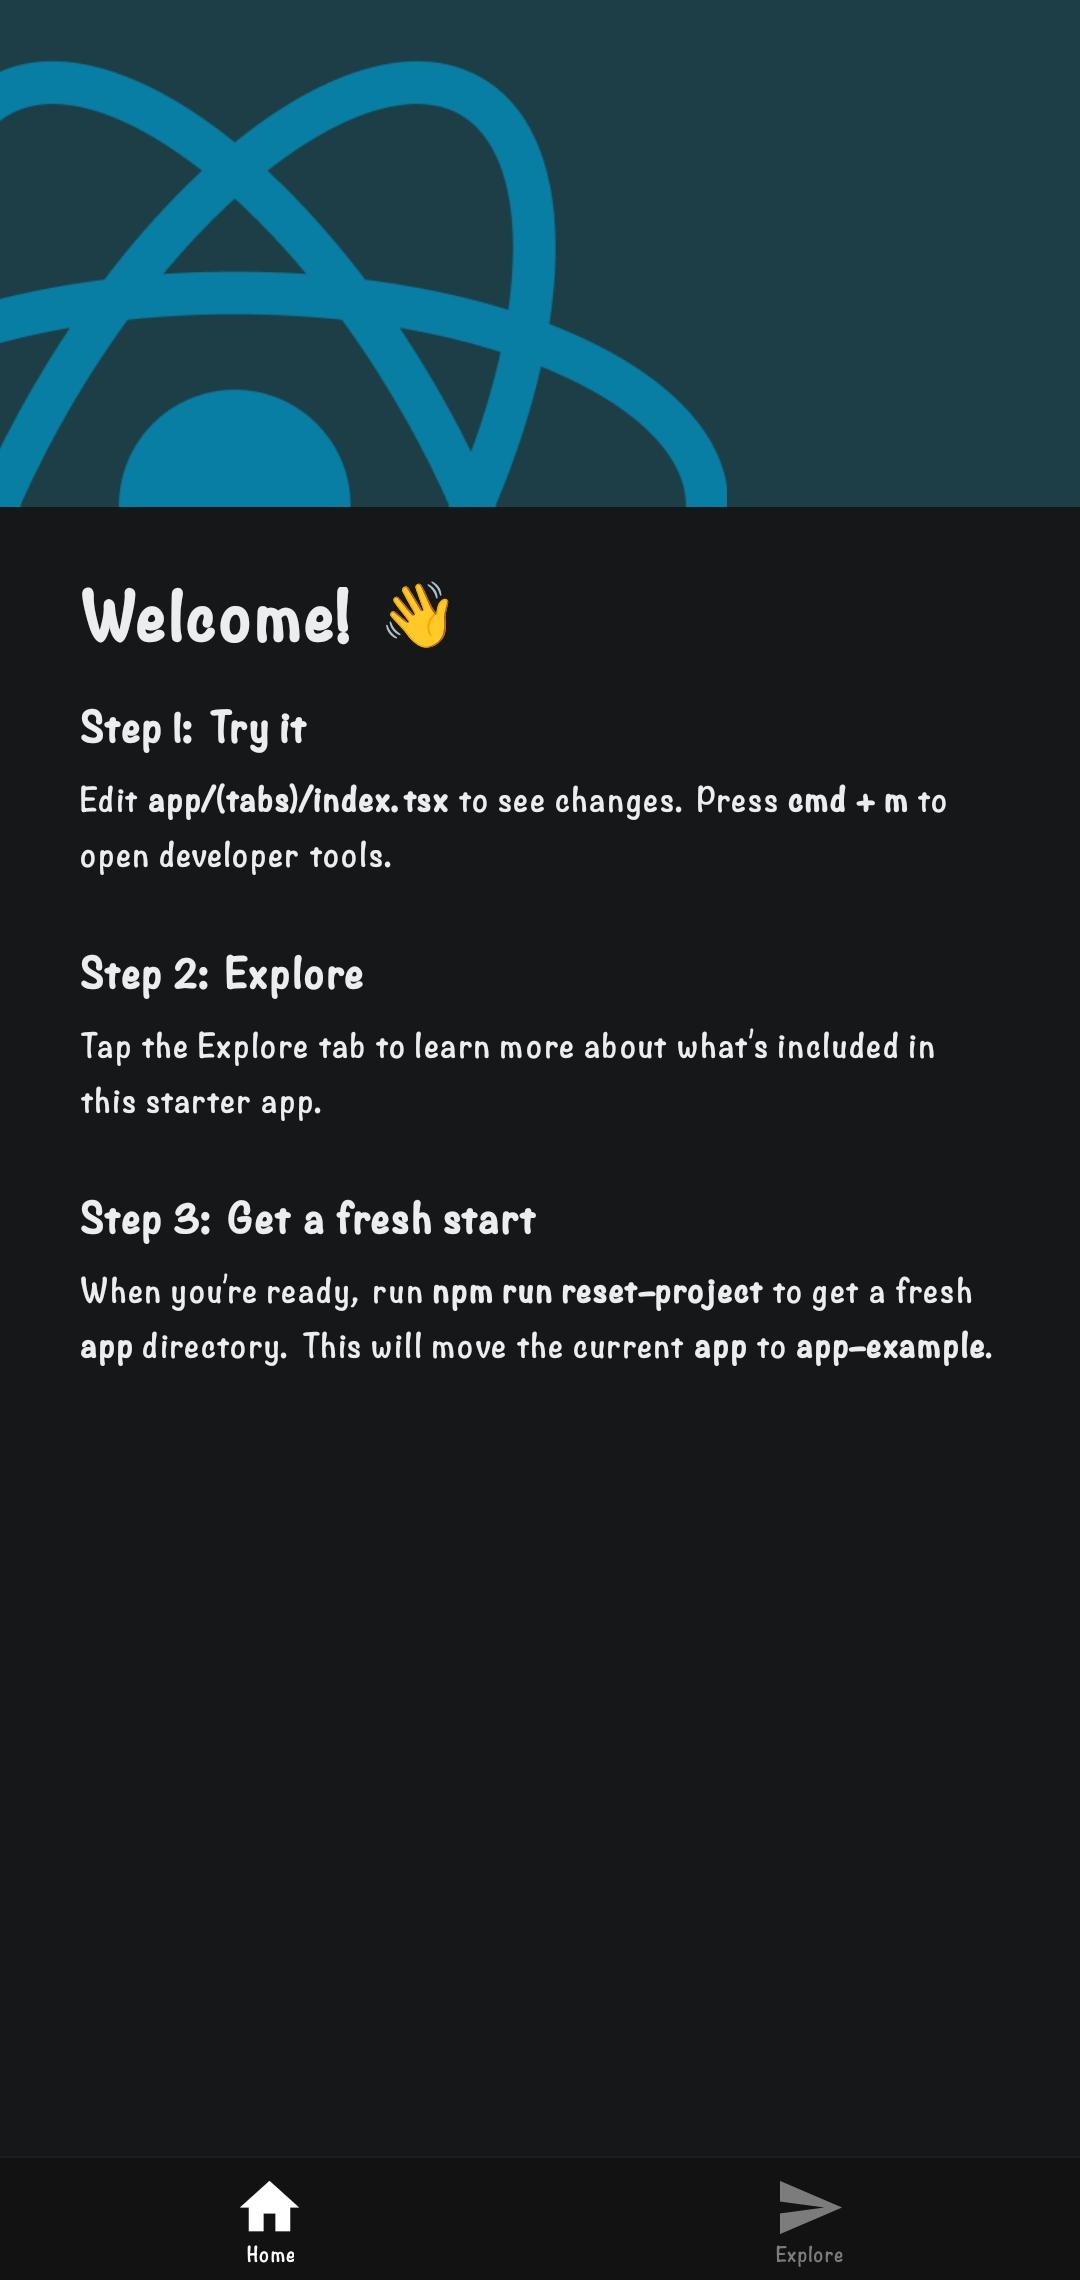
\includegraphics[height=0.45\textheight,keepaspectratio]{img/myapp1.jpeg}
    \caption{Proyecto creado con la plantilla por defecto, con estructura de navegación.}
    \label{fig:myapp1}
\end{figure}

Para apreciar contrastes, generamos una segunda aplicación usando la plantilla en blanco (\textit{blank template}).

\begin{figure}[H]
    \centering
    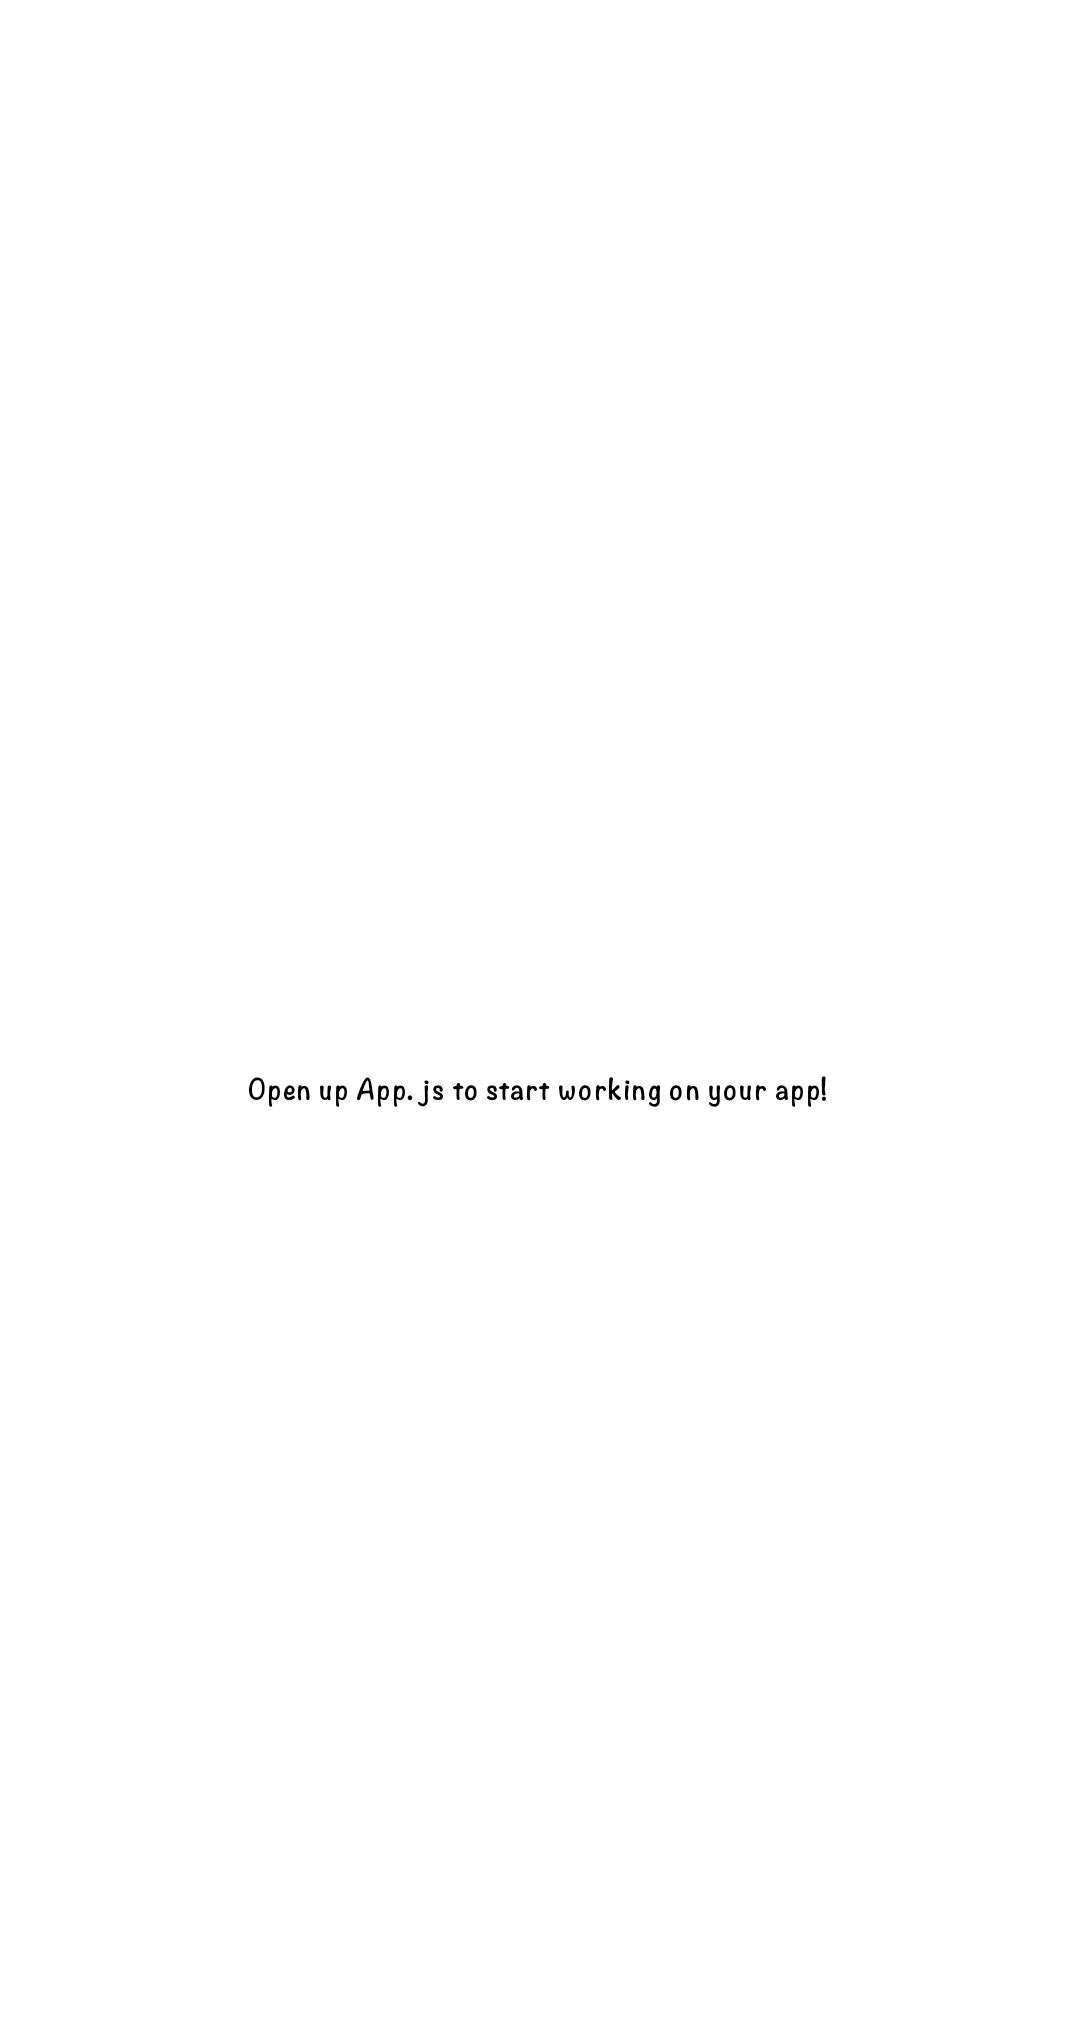
\includegraphics[height=0.45\textheight,keepaspectratio]{img/blank.jpeg}
    \caption{Creación del segundo proyecto bajo la plantilla en blanco (blank template).}
    \label{fig:blank}
\end{figure}

\subsection{Ejecución del proyecto}
Una vez que las dependencias fueron descargadas, ingresamos al directorio de la aplicación generada y levantamos el servidor empaquetador (Metro bundler) mediante:
\begin{verbatim}
npx expo start
\end{verbatim}
\textbf{¿Qué hace este comando?}
Inicia Metro Bundler, un servidor de desarrollo local que compila en tiempo real nuestro código JavaScript. Como evidencia visual en la terminal de la computadora, se muestra un enorme código QR y comandos rápidos (\texttt{j}, \texttt{r}, \texttt{m}, \texttt{w}) que nos sirven para interactuar con la sesión actual.

Adicionalmente, se ejecutó:
\begin{verbatim}
npx expo start --web
\end{verbatim}
\textbf{¿Qué hace este comando?}
Activa la renderización de nuestra aplicación móvil adaptándola a una interfaz web (Expo Web). Abre directamente una pestaña en el navegador de escritorio permitiéndonos visualizar e interactuar con la aplicación simulando una pantalla móvil, pero sin necesidad de un teléfono a la mano.

\begin{figure}[H]
    \centering
    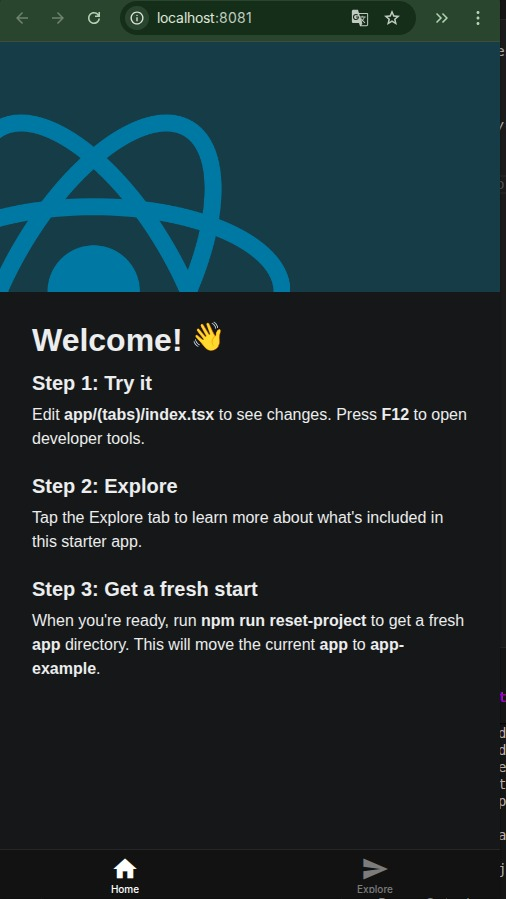
\includegraphics[height=0.45\textheight,keepaspectratio]{img/web.jpeg}
    \caption{Visualización en entorno web local ejecutando \texttt{npx expo start --web}.}
    \label{fig:web}
\end{figure}

\subsection{Uso de Expo Go}
Si bien ejecutar en la web es rápido, para probar funcionalidades reales del teléfono requerimos un dispositivo. Aquí interviene Expo Go, una aplicación descargada desde la Google Play Store o App Store. Al abrirla y escanear el código QR proporcionado en la terminal por el comando \texttt{npx expo start}, la aplicación se compila y carga instantáneamente en nuestro dispositivo de manera inalámbrica (usando la red local).

\textbf{Ventajas de Expo Go:}
\begin{itemize}
    \item Evita la instalación pesada de Android Studio o emuladores lentos.
    \item Ofrece actualización en vivo (\textit{hot reloading}): al guardar cambios en el código de nuestra PC, la pantalla del teléfono se refresca instantáneamente para mostrar el resultado.
\end{itemize}

\subsection{Diferencias observadas entre proyectos}
Durante la práctica, se crearon dos proyectos que evidenciaron diferentes estrategias de inicio:
\begin{itemize}
    \item \textbf{Plantilla Default (\texttt{my-app1}):} Viene con un sistema de enrutamiento integrado, carpetas de componentes, menús de navegación inferior (\textit{tabs}), y recursos iconográficos precargados. Es ideal para aplicaciones que requerirán pantallas múltiples organizadas de manera convencional.
    \item \textbf{Plantilla Blank (\texttt{my-app2}):} Generó un solo archivo principal visible (\texttt{App.js}) con un fondo blanco y un pequeño texto de prueba. No tiene estructura de enrutamiento preconfigurada. Es el enfoque recomendado para cuando se requiere tener absoluto control desde cero sobre cómo estructurar el diseño.
\end{itemize}

\subsection{Estructura de carpetas y archivos}
La exploración de las carpetas nos mostró una estructura universal y estandarizada que React Native y Expo utilizan para organizar el proyecto:
\begin{itemize}
    \item \textbf{node\_modules/}: Carpeta, generalmente pesada, que contiene el código fuente de todas las herramientas y dependencias descargadas por npm. Nunca se modifica manualmente.
    \item \textbf{assets/}: Directorio destinado para colocar recursos estáticos de uso local como las pantallas de carga (splash), logos y archivos de fuentes tipográficas.
    \item \textbf{app/} o \textbf{App.js}: Es el corazón del código; aquí desarrollamos la interfaz de usuario, lógica y componentes.
    \item \textbf{package.json}: Un archivo vital en formato JSON que actúa como el "carnet de identidad" del proyecto. Declara nombre, versión, comandos de ejecución (scripts) y la lista de dependencias instaladas.
    \item \textbf{app.json}: Es el archivo de configuración exclusivo de Expo. Aquí personalizamos el comportamiento intrínseco de la app, color de fondo general, orientaciones permitidas, versión de compilación y el icono que aparecerá en el teléfono.
\end{itemize}

\subsection{Evidencias de ejecución}
Como se visualizó en el entorno de desarrollo local (basado en las ejecuciones registradas), el arranque del empaquetador arrojó información vital en la terminal:
\begin{itemize}
    \item Un bloque grande de caracteres formando un código QR escaneable por el dispositivo móvil a través de la aplicación Expo Go.
    \item La confirmación de que el servidor local estaba activo y escuchando peticiones (por ejemplo, \textit{Metro waiting on localhost:8081}).
    \item Un menú interactivo de atajos de teclado, donde pulsar \texttt{w} abría la versión web, \texttt{a} solicitaba un emulador Android nativo y \texttt{r} forzaba la recarga de toda la aplicación.
\end{itemize}

\section{Resultados obtenidos}
Se logró exitosamente preparar un entorno de desarrollo para programación móvil haciendo uso del framework React Native optimizado por las herramientas de Expo. Se interactuó fluidamente con las interfaces de consola utilizando \texttt{npx} para inicializar el proyecto base con plantillas controladas (tanto en blanco como con pestañas de navegación), y luego ejecutar el empaquetador Metro mediante \texttt{npx expo start}. Las evidencias e imágenes generadas demostraron la correcta configuración de la estructura de archivos y el renderizado funcional de las vistas en el navegador local web.

\section{Conclusión}
A lo largo de esta práctica logré sumergirme profundamente en los flujos modernos del desarrollo móvil multiplataforma. Aprendí que React Native, combinado con la gran capacidad de abstracción de Expo, proporciona una experiencia de desarrollo veloz, donde la brecha entre la escritura del código y su visualización final en el dispositivo es prácticamente instantánea. 

Comprendí que detrás de cada proyecto moderno de JavaScript hay herramientas que trabajan silenciosamente, pero que son fundamentales, como \texttt{npm} y \texttt{npx}. Estas me facilitan la descarga, gestión y ejecución ágil del código; logré que comandos como \texttt{npx create-expo-app} y \texttt{npx expo start} pasaran de ser simples instrucciones memorizadas a convertirse en conceptos fundamentales de empaquetamiento y levantamiento de servidores plenamente asimilados.

Finalmente, pude constatar cómo herramientas de prueba como Expo Go, sumadas a la alternativa de la visualización web, me garantizan un flujo de experimentación continuo que no requiere computadoras con recursos altísimos ni la tediosa y pesada configuración inicial de Android Studio o Xcode, consolidando mi habilidad para iniciar el diseño, arquitectura y codificación de cualquier aplicación móvil desde cero.

\end{document}
